\chapter{Experimenty}

V této kapitole prezentujeme přehled výsledků různých architektur pro extrakci melodie, trénované nad datasetem MedleyDB. Data byla rozdělena na trénovací, validační a testovací množinu tak, aby skladby od jednoho interpreta náležely právě do jedné z množin. Využili jsme existujícího rozdělení používaného v článcích \cite{Bittner2017} a \cite{DBasaranSEssid2018}, validační i testovací výsledky jsou tedy díky tomu porovnatelné s výsledky uvedenými v článcích.

Pro odhad výšky tónů porovnáváme architektury inspirované pracemi \cite{Kim2018}, \cite{Oord2016} a \cite{Bittner2017}. V prvním případě jde o architekturu CREPE původně navrženou pro sledování výšky tónů v jednohlasých nahrávkách. \cite{Oord2016} používají WaveNet složený z dilatovaných konvolucí pro generování lidské řeči. \cite{Bittner2017} používá hlubokou konvoluční síť pro kompletní přepis nahrávek i pro přepis melodie. 

Pro detekci melodie pak srovnáváme jednoduchou metodu práhování a složitější samostatný modul, založený na hlubokých neuronových sítích.

\section{Architektura CREPE}\label{sec:crepe}

První sada experimentů se zakládá na architektuře popsané v článku od \cite{Kim2018} použité pro sledování jednohlasu. Jak blíže popisujeme v kapitole \nameref{cha:souvisejici}, cílem monopitch trackingu je určit konturu základní frekvence melodického nástroje v jednohlasé nahrávce. Tato nahrávka se zpravidla skládá ze směsi čistého signálu hlasu a šumu v pozadí. Pokud však rozšíříme pojem šumu v pozadí tak, aby zahrnoval i melodický doprovod, pak dostáváme polyfonní signál, tedy vstupní signál pro metody extrakce melodie.

Jinými slovy je sledování jednohlasu speciálním případem extrakce melodie a tudíž přinejmenším stojí za zkoušku pokusit se tuto architekturu pro extrakci využít. Mimo to jednohlasé stopy často obsahují přeslech ostatních nástrojů, pokud nahrávka vznikala při společném hraní ve studiu, tudíž by model trénovaný na vícehlasé mixech mohl být robustní vůči tomuto druhu rušení. 

\begin{figure}[h]\centering
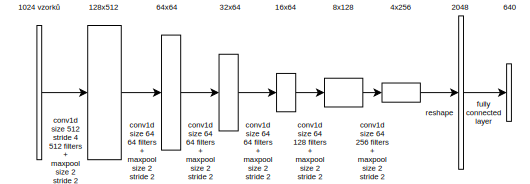
\includegraphics{../img/crepe_arch}
\caption{Diagram architektury CREPE, multiplikační koeficient 16x.}
\label{obr:wavenet_dilated}
\end{figure}

Architektura CREPE se skládá ze šesti konvolučních a pooling vrstev, pro regularizaci používá batch normalization a dropout po každé konvoluční vrstvě, jako nelineární aktivace je použita funkce ReLU. Po konvolucích následuje výstupní plně propojená vrstva, jako finální aktivační funkce je použita sigmoida. Vstupem modelu je okno o velikosti 1024 vzorků jednokanálového audio signálu, převzorkovaného na 16 kHz. Před první konvolucí je signál normalizován tak, aby každé jednotlivé vstupní okno mělo střední hodnotu 0 a směrodatnou odchylku 1. Podrobnější popis modelu je naznačen na obrázku.

Výsledný vektor o 640 složkách aproximuje pravděpodobnostní rozdělení výšky základní frekvence uprostřed vstupního okna, přičemž tento vektor pokrývá rozsah od noty $C_{-1}$ po $G_{9}$, mezi dvěma sousedními predikovanými tóny je vzdálenost 20 centů. Výšky tónů v centech označíme $\cent_1, \cent_2, \dots, \cent_{640}$. Rozsah tedy bezpečně pokrývá obvyklé hudební nástroje a na jednu notu připadá 5 složek (tónů) výsledného vektoru.

    $$\cent(f) = 1200 \log_2{\frac{f}{f_{\mathrm{ref}}}}$$

Pro trénování modelu potřebujeme také cílové diskrétní pravděpodobnostní rozdělení základní frekvence tónu. Jako cílovou pravděpodobnostní funkci použijeme normální rozdělení se střední hodnotou v bodě cílové základní frekvence $\cent(f_{\mathrm{ref}})$ a se směrodatnou odchylkou 25 centů. Toto rozdělení diskretizujeme tak, aby měl cílový vektor stejné dimenze jako odhadovaný.

    $$y_i = \frac{1}{\sqrt{2 \pi \sigma^2}}\exp{(-\frac{(\cent_i - \cent_{\mathrm{ref}})^2}{2 \sigma^2})}$$

Převod z pravděpodobnostní reprezentace výstupního vektoru na konkrétní hodnotu výšky noty provedeme pomocí výpočtu střední hodnoty výstupní distribuce. Jelikož by při výpočtu střední hodnoty ale hodnotu výsledné výšky tónu ovlivňoval i doprovod, který se na výstupním vektoru objevuje, počítáme střední hodnotu pouze z okolí maxima výstupu. Tím zajistíme, že získáme střední hodnotu gaussiánu náležícímu pouze jednomu tónu.

    $$ \left. \hat{\cent} = \sum_{\scaleto{i, \lvert \cent_i - \cent_m \rvert < 50}{8pt}} {\hat{y}_i \cent_i} \middle/ \sum_{\scaleto{i, \lvert \cent_i - \cent_m \rvert < 50}{8pt}} \hat{y}_i \right., m = \mathrm{argmax}_i(\hat{y}_i)$$

Optimalizovaná ztrátová funkce modelu (loss funkce) $\mathcal{L}(\mathbf{y}, \mathbf{\hat{y}})$ se počítá jako vzájemná korelace mezi vektorem cílových pravděpodobností $y$ a výstupním vektorem $\hat{y}$.

    $$\mathcal{L}(\mathbf{y}, \mathbf{\hat{y}}) = \sum_{i = 1}^{640}{(-y_i\log\hat{y}_i - (1-y_i)\log(1-\hat{y_i}))}$$

Optimalizace probíhá pomocí algoritmu Adam \citep{Kingma2014} s parametrem learning rate $0.0002$.

\begin{table}[h!]

\centering
    \begin{tabular}{l@{\hspace{1.5cm}}rrrrrrr}
    \toprule
    {}         &  \textbf{1.}   &  \textbf{2.}  &  \textbf{3.}  &  \textbf{4.}  &  \textbf{5.}   &  \textbf{6.}  &  \textbf{Celk. parametrů} \\
    \midrule
    CREPE 4x   &  128  &  16  &  16  &  16  &  32   &  64  &  $558\,240$ \\
    CREPE 8x   &  256  &  32  &  32  &  32  &  64   &  128 &  $177\,1200$ \\
    CREPE 16x  &  512  &  64  &  64  &  64  &  128  &  256 &  $6\,163\,200$ \\
    \bottomrule
    \end{tabular}

\caption{Počty filtrů v konvolučních vrstvách v architektuře CREPE v závislosti na multiplikačním koeficientu.}\label{tab:crepe_dimensions}

\end{table}

% rozepsat:
% - obhajoba raw signálu

% diskuze:
% - převzorkování na 16kHz
% - normalizace vstupu
% - formulace jako klasifikační úloha, nikoli regresní
% - je lepší odhadovat opravdové pravděpodobnostní rozdělení a nebo jejich škálované? (přijde mi, že kvůli sigmoid aktivaci bude jednodušší 1.0 = Truth, protože ty vstupní logity do sigmoid aktivace můžou být crazyshit velký)
% - crepe model - např. nedává vůbec smysl velikost kernelu 64 v posledních vrstvách, zbytečně se tam přidávají nuly jako padding
% - ukázat vizualizaci první vrstvy

\subsection{Replikace výsledků CREPE}

Abychom ověřili správnost implementace architektury CREPE pro sledování jednohlasu, spustíme model na syntetických, jednohlasých datech MDB-stem-synth, která byla zvěřejněná spolu s článkem od \cite{Salamon2017}.

Na rozdíl od článku \cite{Kim2018}, ve kterém autoři používají pro celkové vyhodnocení architektury pětinásobnou křížovou validaci, jsme použili pouze jednu trénovací a testovací množinu. Zásadní rozdíly mezi implementacemi modelu jsme na základě článku a veřejně dostupného kódu neobjevili.

Po jedné epoše trénování model dosáhl na testovací množině $98.6\%$ přesnosti odhadu výšky. \cite{Kim2018} uvádí přesnost modelu $97\%$. V jejich případě jde o průměrný výsledek pěti nezávislých běhů trénování a testování na různě rozdělených datových množinách. Rozdíl mezi dosaženými přesnostmi přičítáme odlišné evaluační strategii.

\begin{table}[h!]

\centering
    \begin{tabular}{llrr}
    \toprule
    Metrika & Práh & Průměrná hodnota & Hodnota \cite{Kim2018} \\
    \midrule
    RCA & 50 centů & 0.988 & 0.970 \\
    RPA  & 50 centů & 0.986 & 0.967 \\
    RPA  & 25 centů & 0.975 & 0.953 \\
    RPA  & 10 centů & 0.937 & 0.909 \\
    \bottomrule
    \end{tabular}
\caption{Výsledky pokusu o replikaci. Přesnosti nejsou přímo srovnatelné kvůli různým evaluačním strategiím.}\label{tab:crepe_dimensions}

\end{table}

Při replikaci experimentu jsme narazili na důležitost správného promíchání dat. Framework Tensorflow použitý pro trénování promíchává data vždy pomocí bufferu pevné velikosti pro dvojice vstupů a cílových výstupů. V praxi je však potřeba buď nastavit buffer na velikost větší než je celková velikost datasetu, a nebo implementovat vlastní míchání přes všechna dostupná data. Při nedostatečně promíchaných datech totiž trénovací dávka (batch) není reprezentativní pro celý dataset, ale pouze pro jeho podmnožinu, což se negativně projevuje kolísající validační přesností modelu.

\subsection{CREPE pro extrakci melodie}

Jako první experiment extrakce melodie z polyfonních dat spustíme nezměněnou architekturu CREPE, v následujících experimentech se tuto baseline pokusíme překonat. Abychom urychlili trénování následujících experimentů, přesnost určíme pro sítě s různou kapacitou. Pokud se výsledky při různých kapacitách nebudou příliš lišit, můžeme experimenty provádět s architekturou s nižší kapacitou a tím snížit trénovací čas. Kapacity upravíme pomocí multiplikačního koeficientu počtu filtrů u všech konvolučních vrstev, počty filtrů jsou uvedeny v tabulce \ref{tab:crepe_dimensions}.

% TODO: diskuse o under a overfittingu

\begin{table}[h!]

\centering
    % \begin{tabular}{l@{\hspace{1.5cm}}rr}
    % \toprule
    % \textbf{Model}      &  \textbf{RPA}    &  \textbf{RCA} \\
    % \midrule
    % CREPE 4x   &  0.634  &  0.753 \\
    % CREPE 8x   &  0.661  &  0.766 \\
    % CREPE 16x  &  0.666  &  0.771 \\
    % \bottomrule
    % \end{tabular}
% \begin{tabular}{lrrr}
% \toprule
% {} &  Raw Pitch Accuracy &  Raw Chroma Accuracy &  Voicing Accuracy \\
% \thead{Multiplikátor \\ kapacity sítě} &                     &                      &                   \\
% \midrule
% \textbf{4                          } &               0.634 &                0.753 &             0.534 \\
% \textbf{8                          } &               0.661 &                0.766 &             0.534 \\
% \textbf{16                         } &               0.666 &                0.771 &             0.534 \\
% \textbf{32                         } &               0.656 &                0.753 &             0.591 \\
% \bottomrule
% \end{tabular}

\begin{tabular}{rrr}
\toprule
Mult. koef. kapacity &   RPA &   RCA \\
\midrule
                   4 & 0.634 & 0.753 \\
                   8 & 0.661 & 0.766 \\
                  16 & 0.666 & 0.771 \\
                  32 & 0.656 & 0.753 \\
\bottomrule
\end{tabular}
\caption{Výsledky experimentu s různými kapacitami modelu.}\label{tab:crepe_capacity}
\end{table}

\begin{figure}[h]\centering
    \includegraphics[scale=0.6]{../img/figures/crepe_kapacita.pdf}
\caption{Výsledky experimentu s různými kapacitami modelu.}
\label{obr:crepe_capacity}
\end{figure}

Z validačních výsledků po $200\,000$ iteracích (přibližně 6 epoch) vidíme, že se výsledek modelů CREPE 8x a CREPE 16x liší řádově o desetiny procentních bodů. Přitom model s větší kapacitou se trénuje o 35\% delší dobu. Proto pro další srovnávání zvolíme architektury s multiplikačním koeficientem 8, modely s dobrými výsledky případně přetrénujeme s vyšší kapacitou.

\subsection{Vliv rozlišení diskretizace výšky noty}

Otestujeme nastavení granularity výstupního vektoru. V článku \cite{Kim2018} se totiž důvod volby pěti frekvencí na notu nediskutuje. Intuitivně by však mělo vyšší rozlišení spíše pomáhat, důvodem je, že nástroje a zejména lidský hlas se často při hraní odchylují od přesných, definovaných frekvencí hraných not a vyšší rozlišení tyto odchylky může lépe zachytit. Ve výsledku by pak síť s jemnějším výstupem měla dělat méně chyb, kde se skutečná a výstupní hodnota liší o jeden půltón.


\begin{table}[h!]

\centering
    \begin{tabular}{rrr}
    \toprule
    Jemnost diskretizace &   RPA &   RCA \\
    \midrule
                    1 & 0.612 & 0.711 \\
                    3 & 0.653 & 0.760 \\
                    5 & 0.666 & 0.771 \\
                    7 & 0.654 & 0.763 \\
                    9 & 0.658 & 0.760 \\
    \bottomrule
    \end{tabular}

\caption{Architektura CREPE s různou jemností diskretizace.}\label{tab:crepe_diskretizace}

\end{table}

\begin{figure}[h]\centering
    \includegraphics[scale=0.6]{../img/figures/crepe_diskretizace.pdf}
\caption{Architektura CREPE s různou jemností diskretizace.}\label{obr:crepe_diskretizace}
\end{figure}

Jak můžeme pozorovat na výsledných hodnotách, jemná granularita výstupu jednoznačně zlepšuje přesnost sítě. Abychom ověřili domněnku, že vyšší rozlišení pomáhá zmenšit počet chyb o půltón, vytvoříme histogram vzdáleností cílového a odhadovaného tónu. V tomto histogramu by pak měl být zřetelný pokles v příslušných třídách. Podle histogramu se počet chyb o půltón mezi zkoumanými modely liší téměř o polovinu, zlepšení tohoto druhu chyb je tedy podstatné.

\begin{figure}[h]\centering
    \includegraphics[scale=0.6]{../img/figures/crepe_diskretizace_hist.pdf}
\caption{Histogramy vzdálenosti chybného odhadu, výstup prvního modelu má rozlišení 50 centů, výstup druhého 10 centů.}\label{obr:crepe_diskretizace}
\end{figure}

\textcolor{red}{odsud dolů přepsat}

\subsection{Vliv rozptylu cílové pravděpodobnostní distribuce výšky noty}

Podle \cite{Bittner2017} pomáhá cílová distribuce s vyšším rozptylem snížit penalizaci sítě za téměř korektní odhady výšek tónů. Mimo to u dostupných dat často nejsou anotace naprosto perfektní, jisté rozostření hranice anotace tudíž pomáhá i v případě nepřesné cílové anotace, síť pak není tolik penalizována za svou případnou správnou odpověď. 

V článku se však nediskutuje, proč bylo zvoleno nastavení směrodatné odchylky na 20 centů. \cite{Kim2018} používá odchylku 25 centů a není na první pohled zřejmé, jaká je optimální hodnota. Příliš vysoký rozptyl způsobí, že síť bude tolerovat více chyb o půltón, příliš nízký rozptyl naopak penalizuje i téměř správné odhady. Intuitivně se nejlepší nastavení pravděpodobně bude pohybovat kolem používaných 25 centů, jelikož to je hranice chybné klasifikace, na druhou stranu optimální hodnota jistě bude závislá na nastavení rozlišení výstupního vektoru, jelikož nižší rozlišení bude jistě vyžadovat vyšší hodnotu rozptylu (v extrémním případě rozptylu blížícího se k nule a cílové frekvence mimo kvantizační hladiny by vzniklý cílový vektor nemusel obsahovat žádné ostré maximum).

Poznamenám také technický detail, který je důležitý při samotné implementaci. Přestože jsem cílový výstup sítě zadefinoval jako diskrétní pravděpodobnostní rozdělení, při trénování je tento vektor hodnot pronásoben koeficientem tak, aby $\max(\mathbf{y}) = 1.0$ a tedy součet prvků vektoru není roven jedné (a o pravděpodobnostní rozdělení se doopravdy nejedná). Důvodem je použití aktivační funkce *sigmoid* u výstupní vrstvy, která nezaručuje výstup korektního rozdělení. Díky tomu se na výstupu může objevit různé množství stejně pravděpodobných kandidátů na melodii.

Testovaná síť má vstupní okno široké 4096 vzorků, používá multiplikátor kapacity 16x a vstup zpracovává 6 různě širokými konvolučními vrstvami (viz experiment *Vliv násobného rozlišení první konvoluční vrstvy*).


\begin{table}[h!]
\centering
    \begin{tabular}{rrr}
    \toprule
    Rozptyl &   RPA &   RCA \\
    \midrule
    0.000 & 0.657 & 0.759 \\
    0.088 & 0.672 & 0.775 \\
    0.124 & 0.677 & 0.773 \\
    0.177 & 0.689 & 0.784 \\
    0.221 & 0.677 & 0.771 \\
    0.265 & 0.677 & 0.770 \\
    0.354 & 0.669 & 0.773 \\
    0.707 & 0.654 & 0.757 \\
    \bottomrule
    \end{tabular}

\caption{Architektura CREPE, vliv rozptylu cílové distribuce.}\label{tab:crepe_diskretizace}
\end{table}

\begin{figure}[h]\centering
    \includegraphics[scale=0.6]{../img/figures/crepe_rozptyl.pdf}
\caption{Architektura CREPE, vliv rozptylu cílové distribuce.}\label{obr:crepe_diskretizace}
\end{figure}



Z experimentů vyplývá, že optimální směrodatná odchylka se pohybuje kolem hodnoty $0.177$, tedy níže než v porovnávaných pracích. 

% ------
% - cílová distribuce doopravdy není distribuce
% - ty zvláštní testované směrod. odchylky jsou kvůli mé chybné implementaci rozostřování
% - zde můžu přidat obrázek, jak vypadají anotace
%     mám to rozpracované na: http://jirkabalhar.cz:6088/notebooks/bakalarka/algoritmy/ismir2017-deepsalience/deepsalience/out/io_comparison.ipynb#

\subsection{Vliv šířky vstupního okna}

Architektura CREPE byla navržena pro monopitch tracking, dá se předpokládat, že jelikož je v monofonních nahrávkách oproti polyfonním daleko méně (melodického) šumu, není pro určení výšky tónu potřeba větší kontext než použitých 1024 vzorků (při vzorkovací frekvenci 16kHz toto odpovídá 64 milisekundám audia). To ale nemusí platit pro složitější signály, kde by síť mohla z delšího kontextu těžit. Otestujeme tedy vliv většího vstupního okna na výslednou přesnost.


\begin{table}[h!]
\centering
    \begin{tabular}{rrr}
    \toprule
    Šířka vstupního okna &   RPA &   RCA \\
    \midrule
    512 (32 ms)   & 0.634 & 0.748 \\
    1024 (64 ms)  & 0.645 & 0.763 \\
    2048 (128 ms) & 0.648 & 0.760 \\
    4096 (256 ms) & 0.650 & 0.762 \\
    8192 (512 ms) & 0.675 & 0.775 \\
    \bottomrule
    \end{tabular}

\caption{Architektura CREPE, vliv šířky vstupního okna.}\label{tab:crepe_sirka}
\end{table}

\begin{figure}[h]\centering
    \includegraphics[scale=0.6]{../img/figures/crepe_sirka.pdf}
\caption{Architektura CREPE, vliv rozptylu cílové distribuce.}\label{obr:crepe_sirka}
\end{figure}

% TODO: možná by to chtělo taky přetrénovat

% - širší okno se také hodí pro onsety a offsety

\subsection{Vliv násobného rozlišení první konvoluční vrstvy}

Podle \cite{Kim2018} se přesnost CREPE snižuje s výškou tónu. Autoři si tuto skutečnost vysvětlují neschopností modelu generalizovat na barvy a výšky tónů neobsažených v trénovací množině, generalizaci by ale mohla pomoci také úprava modelu. Protože k rozpoznání vyšších frekvencí stačí méně vzorků než pro rozpoznání nižších, mohli bychom se pokusit upravit první konvoluční vrstvu sítě, která tento úkol zastává, a rozdělit ji na množiny různě širokých konvolucí, jejichž kanály následně sloučíme zpět do jednotné vrstvy. To by mělo mít za následek, že rozpoznávání vysokých tónů budou zastávat užší konvoluce a jejich kernel bude jednodušší než široké kernely s vysokou mírou redundance.

První vrstvu s kernelem s 256 filtry (tj. počet filtrů první vrstvy s multiplikátorem 8x, viz první experiment) jsem rozdělil na vícero různě širokých kernelů s menším počtem filtrů, tak aby kapacita sítě zůstala přibližně stejná a sítě byly porovnatelné. 

\begin{table}[h!]
\centering
    \begin{tabular}{lrrrrrrrrr}
    \toprule
    Šířka vrstev & 512 & 256 & 128 & 64 & 32 & 16 & 8  & 4  & Počet parametrů  \\
    Počet vrstev & {} & {} & {} & {} & {} & {} & {}  & {}  & {}  \\
    \midrule
    1                   & 256 &     &     &    &    &    &    &    & 2098880 \\
    2                   & 128 & 128 &     &    &    &    &    &    & 2066112 \\
    3                   & 85  & 85  & 85  &    &    &    &    &    & 2041918 \\
    4                   & 64  & 64  & 64  & 64 &    &    &    &    & 2029248 \\
    5                   & 51  & 51  & 51  & 51 & 51 &    &    &    & 2016350 \\
    6                   & 42  & 42  & 42  & 42 & 42 & 42 &    &    & 2001944 \\
    7                   & 36  & 36  & 36  & 36 & 36 & 36 & 36 &    & 1996184 \\
    8                   & 32  & 32  & 32  & 32 & 32 & 32 & 32 & 32 & 2000448 \\
    \bottomrule
    \end{tabular}
\caption{Počet filtrů prvních vrstev multirezoluční vstupní konvoluční vrstvy.}\label{tab:crepe_velikosti_multirozliseni}
\end{table}

Experiment jsem provedl na síti se vstupním oknem 2048 vzorků, multiplikátorem kapacity 8, 

\begin{table}[h!]
\centering
    \begin{tabular}{rrr}
    \toprule
    Počet konvolučních vrstev &   RPA &   RCA \\
    \midrule
                            1 & 0.669 & 0.779 \\
                            2 & 0.669 & 0.773 \\
                            3 & 0.672 & 0.773 \\
                            4 & 0.674 & 0.778 \\
                            5 & 0.686 & 0.781 \\
                            6 & 0.678 & 0.780 \\
                            7 & 0.677 & 0.779 \\
                            8 & 0.680 & 0.778 \\
    \bottomrule
    \end{tabular}
\caption{Architektura CREPE, vliv multirezoluční vstupní konvoluční vrstvy.}\label{tab:crepe_multirozliseni}
\end{table}

\begin{figure}[h]\centering
    \includegraphics[scale=0.6]{../img/figures/crepe_multirozliseni.pdf}
\caption{Architektura CREPE, vliv multirezoluční vstupní konvoluční vrstvy.}\label{obr:crepe_multirozliseni}
\end{figure}

Zlepšení výsledků se pohybuje v řádu desetin procentních bodů, tedy není příliš vysoké. Zlepšení je nejvíce patrné v případě pěti různě širokých konvolučních vrstev, kde dosahuje $1.3$ procentního bodu. Analýzou výsledků přesnosti podle výšky noty se mi nepodařilo prokázat domněnku, že by konvoluce s více rozlišeními pomáhala u odhadu not vyšších frekvencí. Její přínos je drobný a projevuje se na většině frekvenčních pásem.


\section{Architektura WaveNet}

Generativní model WaveNet popsaný týmem \cite{Oord2016} je architektura navržená pro generování zvukového signálu. Autoři však v článku zmiňují, že se architekturu pokusili využít i pro převod mluvené řeči na text (dataset TIMIT), a podařilo se jim dosáhnout výsledků srovnatelných se state-of-the-art. Architektura spočívá ve vrstvení dilatovaných konvolucí s rozšiřujícím se rozsahem. Díky exponenciálně rostoucím dilatacím se také exponenciálně zvětšuje receptivní pole jednotlivých konvolučních vrstev. Díky této vlastnosti pak například stačí pro pokrytí 1024 vzorků vstupu pouze 9 vrstev s šířkou kernelu 2 a dilatacemi 1,2,4,8 ... 512. Pokud bychom stejného receptivního pole chtěli dosáhnout pomocí obvyklých konvolucí počet potřebných vrstev by byl lineární vzhledem k šířce pole. Vrstvení konvolucí je porovnáno na obrázcích \ref{obr:wavenet_conv} a \ref{obr:wavenet_dilated}. Síť tedy velmi snadno pokryje široký kontext, což je vlastnost, která je pro zpracování zvukového signálu užitečná.

\begin{figure}[h]\centering
\includegraphics{../img/wavenet_konvoluce}
\caption{Vrstvení obyčejných konvolucí s lineárně rozšiřovaným dosahem, obrázek převzat z \cite{Oord2016}.}
\label{obr:wavenet_conv}
\end{figure}

\begin{figure}[h]\centering
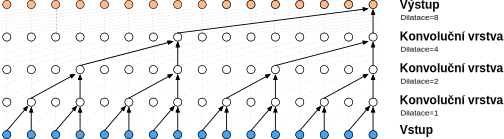
\includegraphics{../img/wavenet_dilatace_konvoluce}
\caption{Vrstvení dilatovaných konvolucí s exponenciálně rozšiřovaným dosahem, obrázek převzat z \cite{Oord2016}.}
\label{obr:wavenet_dilated}
\end{figure}

Síť se pro Music Information Retrieval úlohy od svého zveřejnění příliš neuchytila. Její použití se v oblasti hudby se omezuje na generativní úlohy (\cite{Hawthorne2018a}, \cite{Yang2017}, \cite{Engel2017} a další), případně pro source-separation \citep{Stoller2018}. Jediný publikovaný pokus s použitím architektury WaveNet pro příbuznou úlohu kompletního automatického přepisu podnikli \cite{Martak2018} s použitím datasetu MusicNet. Jejich model však netestovali na standardních evaluačních datasetech ze soutěže MIREX, tudíž není zřejmé, jakých výsledků v porovnání s existujícími metodami autoři dosáhli.



\begin{figure}[h]\centering
\includegraphics{../img/wavenet_arch}
\caption{Architektura WaveNet upravená pro kompletní přepis skladeb, upraveno na základě \cite{Martak2018}.}
\label{obr:wavenet_arch}
\end{figure}

\subsection{Baseline na základě \cite{Martak2018}}

% python -u wavenet.py --evaluate --filter_width 2 --initial_filter_width 2 --max_dilation 512 --stack_number 2 --residual_channels 128 --skip_channels 128 \
%     --batch_size 20 --min_note 0 --note_range 128 --bins_per_semitone 1 --annotation_smoothing 0 \
%     --iterations 100000 --learning_rate_decay_steps 10000 --learning_rate_decay 0.8 --annotations_per_window 5 --context_width 2100 --use_biases --frame_width 160 \
%     --skip add --postprocessing "conv_f128_k1_s1_Psame_arelu--conv_f128_k1_s1_Psame--avgpool_p160_s160_Psame"


Pro extrakci melodie využijeme jako výchozí model upravenou architekturu od \cite{Martak2018}, jejíž struktura je naznačena na obrázku \ref{obr:wavenet_arch}. Vstupem je okno velikosti 4894 vzorků audia převzorkovaného na $16\,\rm kHz$, toto okno nejprve zpracujeme standardní konvoluční vrstvou s šířkou kernelu 2 a 128 výstupními kanály, takto zpracovaný signál dále prochází dvěma bloky po desíti vrstvách, které obsahují dilatované konvoluce. Vrstvy obsahují dvě dilatované konvoluce, jednu s aktivací hyperbolickým tangens a jednu s aktivační funkcí sigmoid. Výstupy těchto konvolucí jsou po složkách vynásobeny, díky čemuž konvoluce s aktivací sigmoid funguje jako nastavitelná propust signálu (Gated activation unit, \cite{Oord2016a}), poté je výstup opět zpracován dvěmi konvolucemi, tentokrát se šířkou kernelu 1x1. Výstup první sečteme s původním vstupem celé vrstvy (jedná se o residuální propojení poprvé popsané v práci \cite{He2015}) a zpracujeme ho nadcházející vrstvou. Výstup druhé konvoluce (autoři tuto cestu nazývají \emph{skip propojení}) zařadíme mezi výstupy skip propojení všech ostatních vrstev.

Pro výpočet odhadů výšky tónu sečteme všechna skip propojení, tento součet zpracujeme dvěma konvolucemi, druhá z nich má na výstupu 128 kanálů zpracovaných sigmoidou, což odpovídá rozsahu odhadovaných not. Jelikož všechny popsané transformace zachovávají šířku vstupu, dostáváme po této konvoluci odhady výšek not pro každý vstupní vzorek zvuku, taková anotace je zbytečně podrobná, tudíž výsledné anotace podvzorkujeme pomocí pooling vrstvy počítající průměr hodnot.

\begin{figure}[h]\centering
    \includegraphics[scale=0.6]{../img/figures/wavenet_overfit}
    \caption{Vývoj ztrátové funkce při učení architektury \cite{Martak2018} pro extrakci melodie. Zatímco hodnoty pro trénovací množinu mají klesající tendenci, hodnoty na validační množině rostou, síť se velmi rychle přeučuje.}\label{obr:wavenet_overfit}
\end{figure}

Po $20\,000$ iteracích s velikostí dávky 20 a parametrem learning rate $0.001$ síť dosahuje na validačních datech přesnost odhadu tónu $0.583$ (RPA) a přesnost odhadu tónu nezávisle na oktávě $0.692$ (RCA). V porovnání s výsledky architektury CREPE jsou tyto výsledky výrazně nižší, krom toho učení sítě trvá velmi dlouho (14 minut na 1000 iterací), zejména kvůli obrovské kapacitě a topologické komplexitě modelu ($2\,009\,728$ trénovatelných parametrů). Veliká kapacita modelu také způsobuje přeučení sítě (viz \ref{obr:wavenet_overfit}), pokusíme se tedy zrychlit trénování a zabránit přeučení výrazným snížením počtu filtrů dilatačních a skip propojení ze 128 na 16, a použitím pouze jednoho dilatačního bloku. Také snížíme velikost trénovací dávky na 8 pro další zrychlení učení. Nová síť obsahuje 10 vrstev s dilatacemi $(1, 2, 4, 8, \dots, 512)$, a tedy $34\,736$ parametrů a dosahuje RPA $0.598$ a RCA $0.696$ po $100\,000$ iteracích při rychlosti trénování 30 sekund na 1000 iterací. Síť tedy dosahuje stejných výsledků ve výrazně kratším čase.

Z předchozích experimentů na architektuře CREPE víme, že jemnější výstupní reprezentace pomáhá snížit počet chyb o půltón, upravíme tedy síť tak, aby na jeden půltón připadalo 5 výstupních složek vektoru, zmenšíme výstupní frekvenční rozsah a hodnoty cílového vektoru změníme z ostré predikce konkrétního tónu na \uv{rozmlžený} gaussián se směrodatnou odchylkou $18\,\rm centů$ (pro podrobnější popis viz \ref{sec:crepe}). Síť po této úpravě dosahuje RPA 0.629 a RCA 0.731 po $100\,000$ iteracích. 

\begin{figure}[h]\centering
    \includegraphics[scale=0.8]{../img/wavenet_lastlayer}
    \caption{Úprava posledních vrstev WaveNet architektury.}\label{obr:wavenet_lastlayer}
\end{figure}

Předběžným hledáním výchozí architektury pro nadcházející sadu experimentů jsme došli k následujícím úpravám. Dilatované konvoluce ve všech vrstvách mají šířku 3 místo 2, jejich vstup tedy závisí na všech okolních vzorcích, nikoli jen na předchozích, jak je naznačeno na obrázku \ref{obr:wavenet_dilated}. Dále jsme odstranili konvoluční vrstvu, která zpracovává vstup, ten je tedy přímo zpracován dilatačním blokem. Ze skip propojení se zpracovává pouze poslední, nedochází ke sčítání všech, což je úprava, kterou pro přepis řeči používají původní autoři článku WaveNet \cite{Oord2016}. Tento výstup je následně zpracován pooling vrstvou a dvěmi konvolucemi se skoky (stride), viz obrázek \ref{obr:wavenet_lastlayer}. Tato síť dosahuje RPA 0.655 a RCA 0.759 po $100\,000$ iteracích a je základem pro následující experimenty.

\subsection{Vliv počtu filtrů dilatačních vrstev a skip propojení}

Jedním ze zásadních faktorů ovlivňujících kapacitu sítě je počet filtrů dilatačních vrstev a skip propojení. Tyto kanály nesou informaci o vzorku a jeho okolí, v závislosti na vrstvě dilatace. Výstup poslední vrstvy má tedy délku počtu vstupních vzorků 2848 a 16 kanálů. Každý výstupní vzorek nese informaci o svém okolí délky 2047. Podobně jako v případě architektury CREPE nalezneme vhodnou kapacitu sítě tak, aby nedocházelo k přeučení (overfitting) ani k nedoučení (underfitting) na trénovací množině.

\begin{table}[h!]
\centering
    \begin{tabular}{rrr}
    \toprule
    Počet kanálů &   RPA &   RCA \\
    \midrule
            4 & 0.609 & 0.714 \\
            8 & 0.628 & 0.739 \\
            16 & 0.655 & 0.759 \\
            24 & 0.665 & 0.764 \\
            32 & 0.671 & 0.771 \\
            40 & 0.667 & 0.766 \\
            48 & 0.667 & 0.764 \\
    \bottomrule
    \end{tabular}

\caption{Architektura WaveNet, vliv počtu filtrů dilatačních vrstev a skip propojení.}\label{tab:wavenet_dil_skip_channels}
\end{table}

\begin{figure}[h]\centering
    \includegraphics[scale=0.6]{../img/figures/wavenet_dil_skip_channels.pdf}
\caption{Architektura WaveNet, vliv počtu filtrů dilatačních vrstev a skip propojení.}\label{obr:wavenet_dil_skip_channels}
\end{figure}

Na základě výsledků volíme pro další experimenty nastavení 16 filtrů pro dilatované konvoluce a skip propojení. Při nastavení 24 a více filtrů dosažená přesnost sítě stagnuje, 16 filtrů je kompromisem z hlediska rychlosti trénování.

\subsection{Systematické prohledávání počtu dilatačních vrstev a bloků}

Velikost zpracovávaného kontextu lze v architektuře WaveNet ovlivnit třemi různými hyperparametry. Jde o počet vrstev v bloku $n_{\mathrm{layers}}$, počet dilatačních bloků poskládaných nad sebou $n_{\mathrm{stacks}}$ a šířka kernelu dilatací $n_{\mathrm{width}}$. Přesně lze dosah vypočítat jako 

    $$\mathrm{receptive\_field} = (n_{\mathrm{width}}-1)\cdot(\sum_d^{n_{\mathrm{layers}}}{2^{(d-1)}})\cdot n_{\mathrm{stacks}}+1$$

Dosud jsme testovali sítě s jedním blokem o deseti vrstvách s dilatacemi $(1,2,4,8,16,\dots,512)$ s šířkou konvolucí 3, její dosah je tedy 2047 vzorků. Systematickým prohledáváním prozkoumáme vliv delšího kontextu měněného pomocí $n_{\mathrm{layers}}$ a $n_{\mathrm{stacks}}$. Při vyhodnocování experimentu je nutné vzít v úvahu, že přidání nové vrstvy, případně celého nového bloku, zároveň zvyšuje kapacitu modelu, což také ovlivňuje výslednou přesnost modelu. Šířky kontextu a kapacity jsou uvedené v tabulce \ref{tab:wavenet_dilation_width_numbers}.

V architektuře modelu jsme pro tento experiment provedli změnu ve zpracování skip propojení. V této sadě se nebere poslední skip propojení, nýbrž všechna se spojí v ose kanálů a slouží jako vstup pro následující pooling vrstvu a konvoluci. Z toho důvodu má model mnohem více parametrů, na druhou stranu je zajištěno, že poslední vrstvy mohou využít informace ze všech skip spojení k odhadu výšek. Na základě srovnání tréninkové a validační ztrátové funkce však modely nevykazují známky přeučení.

\begin{table}[h!]
\centering
    \begin{tabular}{lrrrrr}
    \toprule
    Max. dilatace & 64 & 128 & 256 & 512 & 1024 \\
    Počet bloků   & {} & {}  & {}  & {}  & {}  \\
    \midrule
    1 (dosah) & 255  & 511  & 1023 & 2047 & 4095 \\
    1 (kapacita) & $4\,483\,644$  & $4\,531\,836$ & $4\,580\,028$ & $4\,628\,220$ & $4\,676\,412$ \\
    2 (dosah) & 509  & 1021 & 2045 & 4093 & 8189 \\
    2 (kapacita) & $4\,820\,988$  & $4\,917\,372$ & $5\,013\,756$ & $5\,110\,140$ & $5\,206\,524$ \\
    3 (dosah) & 763  & 1531 & 3067 & 6139 & $12\,283$ \\
    3 (kapacita) & $5\,158\,332$  & $5\,302\,908$ & $5\,447\,484$ & $5\,592\,060$ & $5\,736\,636$ \\
    4 (dosah) & 1017 & 2041 & 4089 & 8185 & --- \\
    4 (kapacita) & $5\,495\,676$  & $5\,688\,444$ & $5\,881\,212$ & $6\,073\,980$ & --- \\
    \bottomrule
    \end{tabular}
\caption{Architektura WaveNet, dosah a kapacita v závislosti na dilatačních počtu vrstev a bloků.}\label{tab:wavenet_dilation_width_numbers}
\end{table}

\begin{figure}[h]\centering
    \includegraphics[scale=0.5]{../img/figures/wavenet_stacks_gridsearch.pdf}
\caption{Architektura WaveNet, systematické prohledávání počtu dilatačních vrstev a bloků, vlevo hodnoty RPA, vpravo RCA.}\label{obr:wavenet_stacks_gridsearch}
\end{figure}

Z tabulky lze dojít k pozorování, že přidávání počtu vrstev zvyšuje výslednou přesnost víceméně vždy, to neplatí o počtu bloků, u kterých se zdá, že nejvhodnější počet je 2. Pokud se zaměříme na srovnání výsledků s podobným dosahem, zdá se že výsledky jsou poměrně podobné, zejména pro širší dosahy, pro kratší se zdá lepší využít spíše více vrstev než více bloků.

\subsection{Vliv velikosti šířky kernelu dilatací}

Jiným způsobem, jak zvýšit velikost zpracovávaného kontextu, je volba velikosti šířky kernelu dilatací $n_{\mathrm{width}}$. Provedeme čtyři experimenty s různou šířkou. Šířka 2 je zvolena v původním článku z toho důvodu, že konvoluce se tím stávají \uv{kauzální} --- jejich výstup závisí pouze na vzorcích před nimi (viz obrázky \ref{obr:wavenet_conv}, \ref{obr:wavenet_dilated}). To je výhodné pro generativní úlohy, u kterých chceme, aby hodnota nového generovaného vzorku v audio signálu nezávisela na budoucích, zatím neexistujících vzorkách. U klasifikačních úloh takto omezeni nejsme, tudíž můžeme s nastavením experimentovat. 

\begin{table}[h!]
\centering
    \begin{tabular}{rrr}
    \toprule
    Šířka kernelu dilatací &   RPA &   RCA \\
    \midrule
                        2 & 0.649 & 0.754 \\
                        3 & 0.648 & 0.755 \\
                        4 & 0.656 & 0.759 \\
                        5 & 0.645 & 0.756 \\
    \bottomrule
    \end{tabular}
\caption{Architektura WaveNet, vliv velikosti šířky kernelu dilatací.}\label{tab:wavenet_dilation_width}
\end{table}

\begin{figure}[h]\centering
    \includegraphics[scale=0.6]{../img/figures/wavenet_dilation_width.pdf}
\caption{Architektura WaveNet, vliv velikosti šířky kernelu dilatací.}\label{obr:wavenet_dilation_width}
\end{figure}

Z tabulky \ref{tab:wavenet_dilation_width} a grafu \ref{obr:wavenet_dilation_width} vyplývá, že tato síť při změnách šířky kernelu dilatace svou výslednou přesnost na validačních datech nemění.

\subsection{Vliv výstupní transformace skip propojení}

Volba transformace skip propojení se v článku týmu \cite{Oord2016} nediskutuje, \cite{Martak2018} také přejímají součet všech skip výstupů Vyzkoušíme proto dvě další možnosti práce se skip propojeními - výběr posledního skip propojení a dále konkatenace všech skip propojení do mnohakanálového výstupu. V případě výběru posledního či součtu jde o transformace, které lze popsat konvolucí nad konkatenovanými skip propojeními. Dalo by se tedy říct, že výběr a součet jsou v tomto případě speciálními případy konkatenace výstupů. Výběr poslední vrstvy také znamená, že nejsou potřeba předchozí skip propojení, což urychluje trénování.

\begin{table}[h!]
\centering
    \begin{tabular}{lrr}
    \toprule
    Transf. skip vrstev &   RPA &   RCA \\
    \midrule
            Konkatenace & 0.654 & 0.754 \\
            Poslední & 0.651 & 0.754 \\
                Součet & 0.646 & 0.753 \\
    \bottomrule
    \end{tabular}

\caption{Architektura WaveNet, vliv výstupní transformace skip propojení.}\label{tab:wavenet_skip_reduction}
\end{table}

\begin{figure}[h]\centering
    \includegraphics[scale=0.6]{../img/figures/wavenet_skip_reduction.pdf}
\caption{Architektura WaveNet, vliv výstupní transformace skip propojení.}\label{obr:wavenet_skip_reduction}
\end{figure}

Všechny tři transformace vedou ke stejné přesnosti. Síť tedy netěží z větších možností práce s dřívejšími vrstvami a nejdůležitejší informace se objevují až na vrchu bloků dilatovaných konvolucí.

\subsection{Vliv velikosti první konvoluce}

\cite{Oord2016} používá pro předzpracování zvukového signálu obvyklou konvoluci, nespecifikuje však její šířku. Veřejná implementace architektury WaveNet pracuje s šířkou 32 \footnote{\url{https://github.com/ibab/tensorflow-wavenet/blob/master/wavenet_params.json}}. \cite{Martak2018} používají šířku 2, čímž fakticky jen duplikují první dilatační vrstvu. První vrstva může sloužit jako banka filtrů, podobně jako první vrstva v architektuře CREPE, pro tento účel však musí být široká minimálně 512 vzorků, aby mohla zachytit periodu i té nejnižší frekvence ve výstupním rozsahu. 

\textcolor{red}{vizualizace první vrstvy? Co tam vlastně může být, když pomáhá šestnácti samplová konvoluce?}

\begin{table}[h!]
\centering
    \begin{tabular}{rrr}
    \toprule
    Velikost první vrstvy &   RPA &   RCA \\
    \midrule
                        0 & 0.648 & 0.755 \\
                        8 & 0.663 & 0.762 \\
                    16 & 0.661 & 0.765 \\
                    32 & 0.654 & 0.754 \\
                    64 & 0.643 & 0.756 \\
                    256 & 0.609 & 0.735 \\
                    1024 & 0.601 & 0.734 \\
    \bottomrule
    \end{tabular}
\caption{Architektura WaveNet, vliv velikosti první konvoluce.}\label{tab:wavenet_first_layer}
\end{table}

\begin{figure}[h]\centering
    \includegraphics[scale=0.6]{../img/figures/wavenet_first_layer.pdf}
\caption{Architektura WaveNet, vliv velikosti první konvoluce.}\label{obr:wavenet_first_layer}
\end{figure}

\textcolor{red}{TODO: Dopsat vyhodnocení}

\subsection{Vliv návrhu posledních vrstev}

\begin{table}[h!]
\centering
\caption{Architektura WaveNet, vliv návrhu posledních vrstev.}\label{tab:wavenet_output_transform}
\end{table}

\begin{figure}[h]\centering
    \includegraphics[scale=0.6]{../img/figures/wavenet_output_transform.pdf}
\caption{Architektura WaveNet, vliv návrhu posledních vrstev.}\label{obr:wavenet_output_transform}
\end{figure}

